\begin{frame}{Status}
\begin{block}{Last milestone}
\begin{itemize}
	\item[\textcolor{green}{\Checkmark}] Manual voxelization using CVMLCPP
	\item[\textcolor{green}{\Checkmark}] "Hard coded" script for ToPy input
	\item[\textcolor{green}{\Checkmark}] Topology optimized geometry using ToPy
	\item[\textcolor{red}{\XSolidBrush}] Recognition of boundary conditions
\end{itemize}
\end{block}
\begin{block}{Today}
\begin{itemize}
	\item[\textcolor{green}{\Checkmark}] Voxelization with OpenCascade
	\item[\textcolor{green}{\Checkmark}] Extraction of loads, fixtures and active elements through colouring
	\item[\textcolor{green}{\Checkmark}] Automatic "one click" pipeline to surface reconstruction
\end{itemize}
\end{block}
\end{frame}

\subsection{Internal structure}
%\begin{frame}{The user's view DRAFT}
%\begin{minipage}{0.65\textwidth}
%\begin{overlayarea}{\textwidth}{.9\textheight}
%\begin{itemize}
%	\item Model geometry in favorite CAD tool (FreeCAD, OpenSCAD)
%	\item Colour faces where boundary conditions are applied
%	\begin{itemize}
%		\item[\textcolor{red}{Red}] Fixture
%		\item[\textcolor{green}{Green}] Active
%		\item[\textcolor{red}{R}\textcolor{green}{G}\textcolor{blue}{B}] RGB value in $[0 \leq \text{\textcolor{red}{R}} < 255,0 \leq \text{\textcolor{green}{G}} < 255,0 \leq \text{\textcolor{blue}{B}} < 255]$ for load vector
%	\end{itemize}
%	\item Save model as \textit{STEP with Colours} and \textit{IGES with Colours}
%	\item Run \textit{\textbf{NAME}} \textit{filename} \textit{force{\_}scaling}
%\end{itemize}
%\begin{figure}[htp]
%\centering
%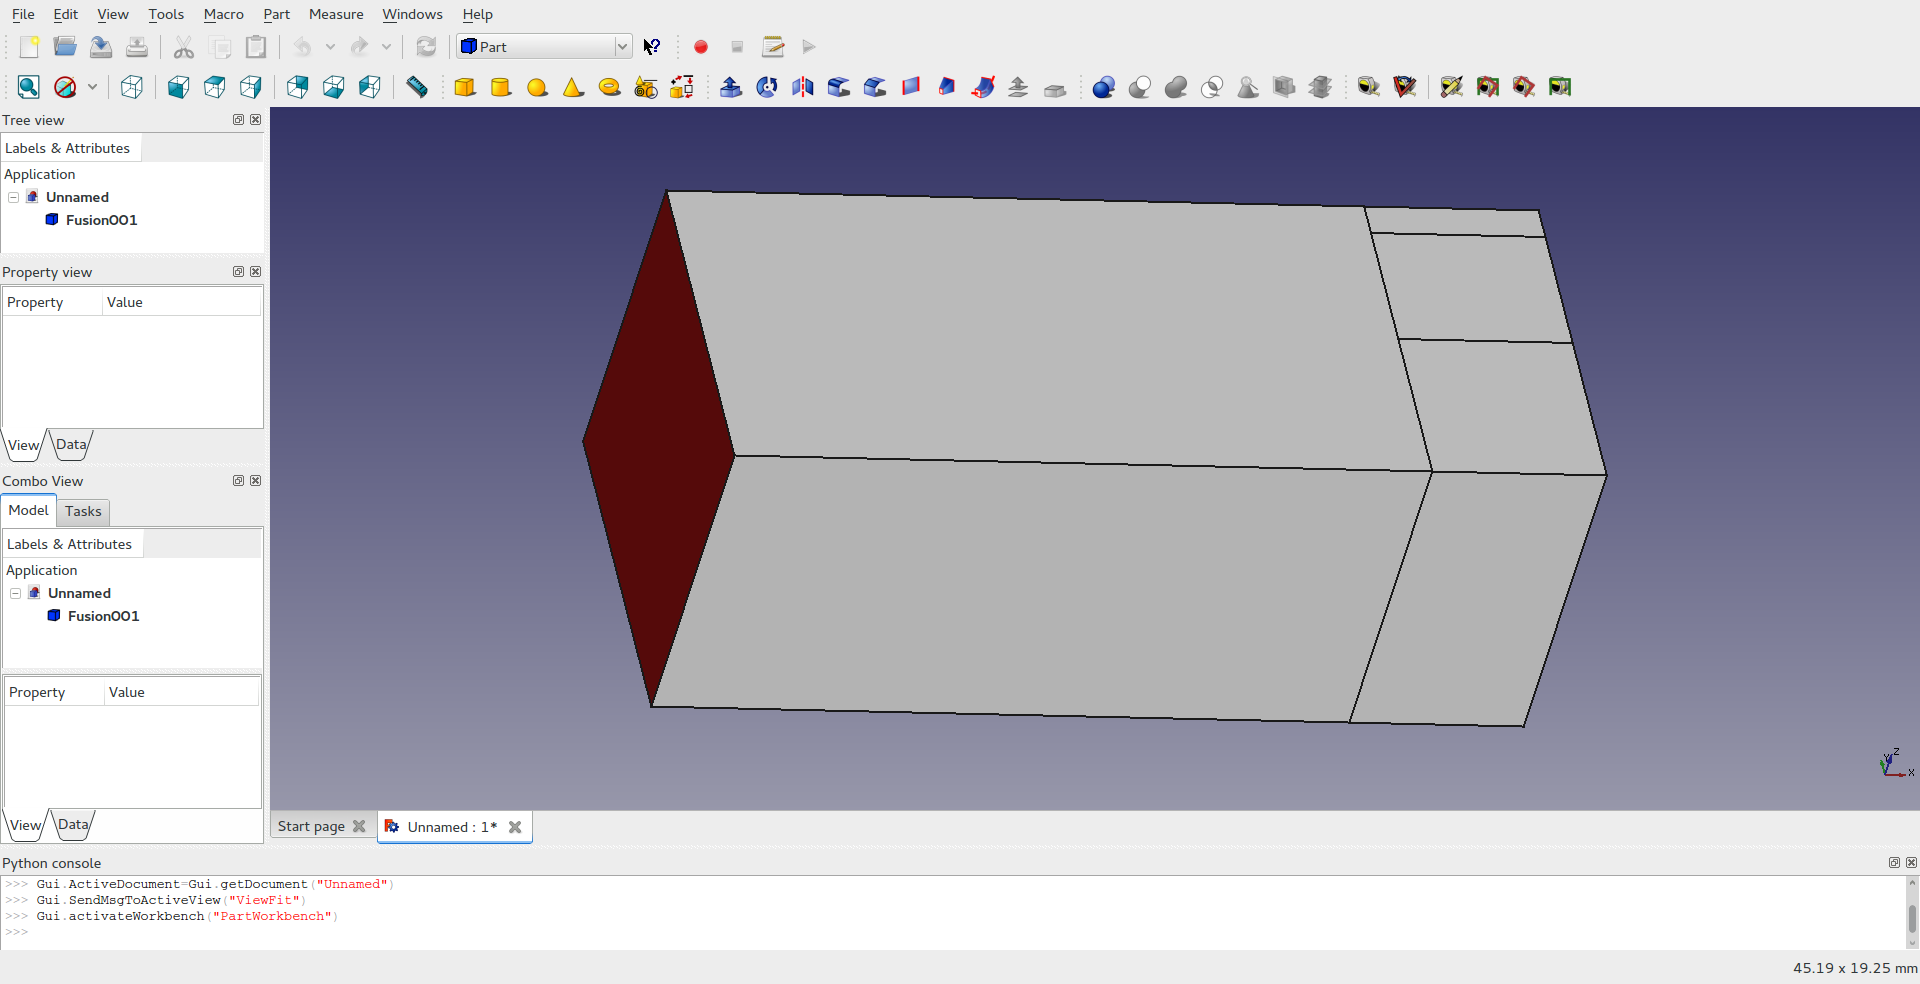
\includegraphics[width=.3\textwidth]{Pictures/TopOp/CantileverFCAD1.png}\hfill
%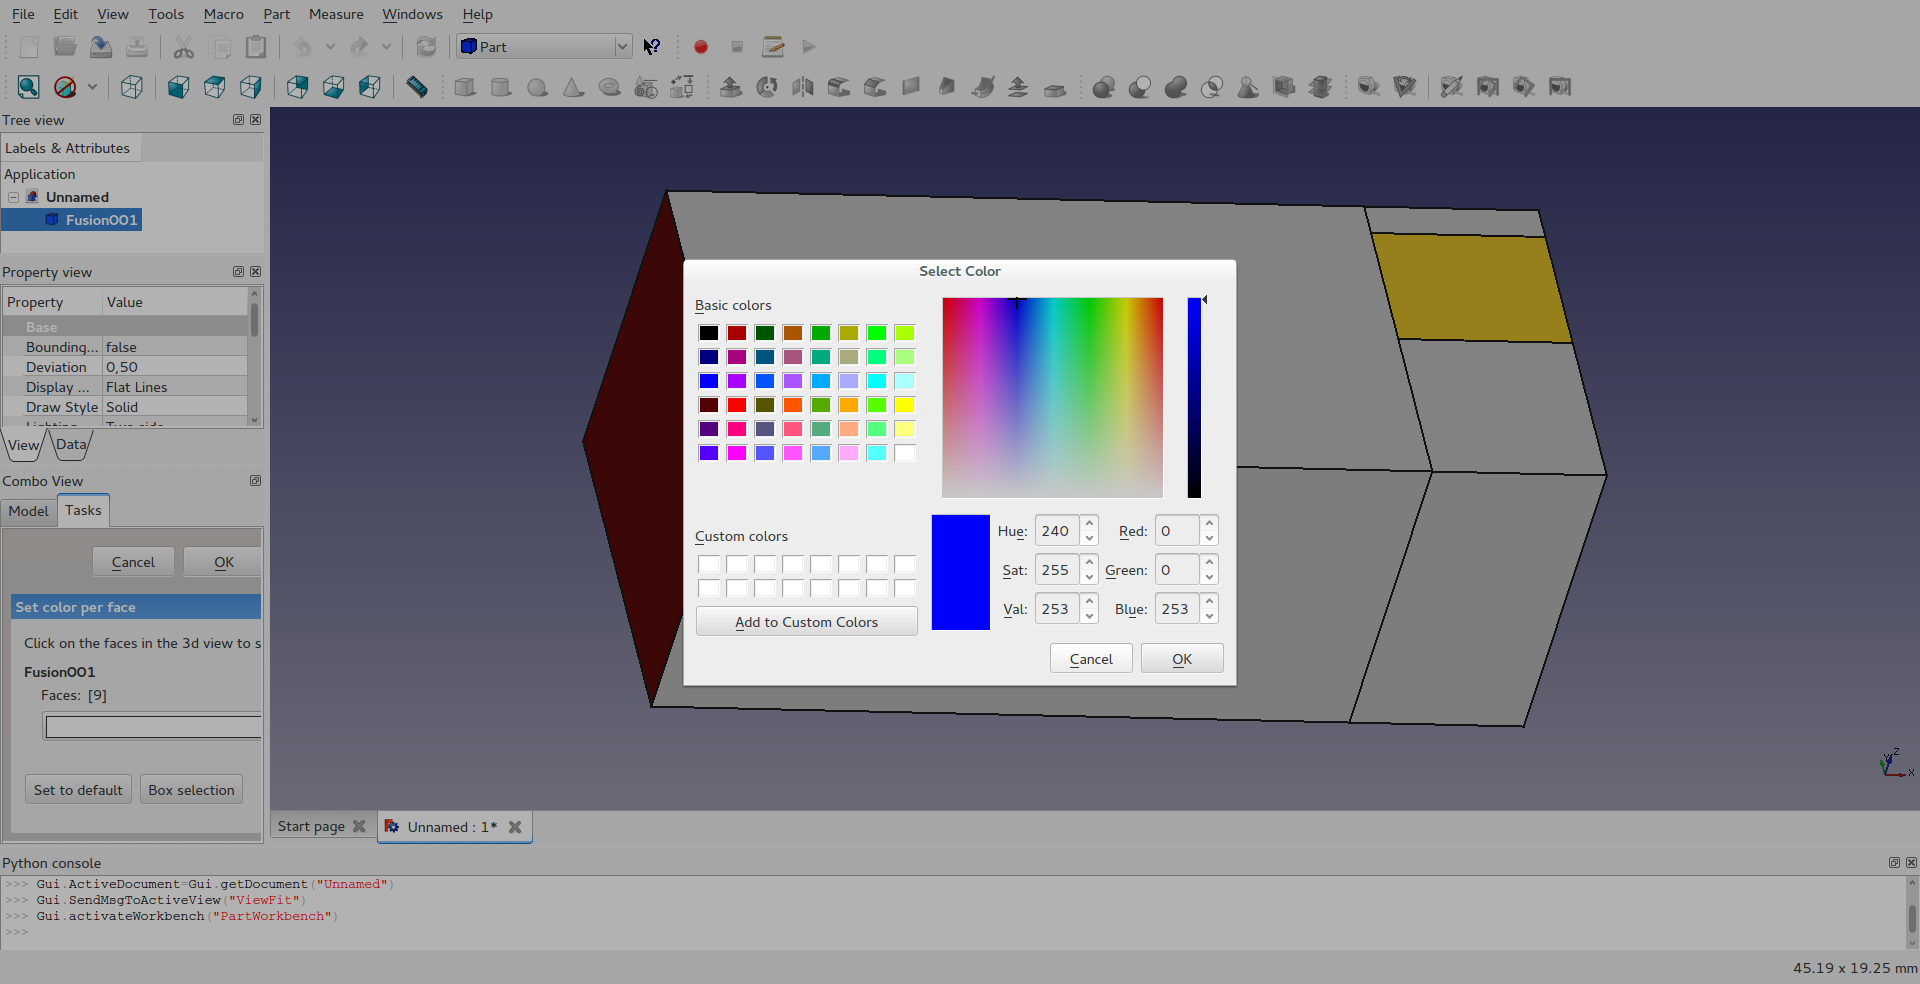
\includegraphics[width=.3\textwidth]{Pictures/TopOp/CantileverFCAD2.png}\hfill
%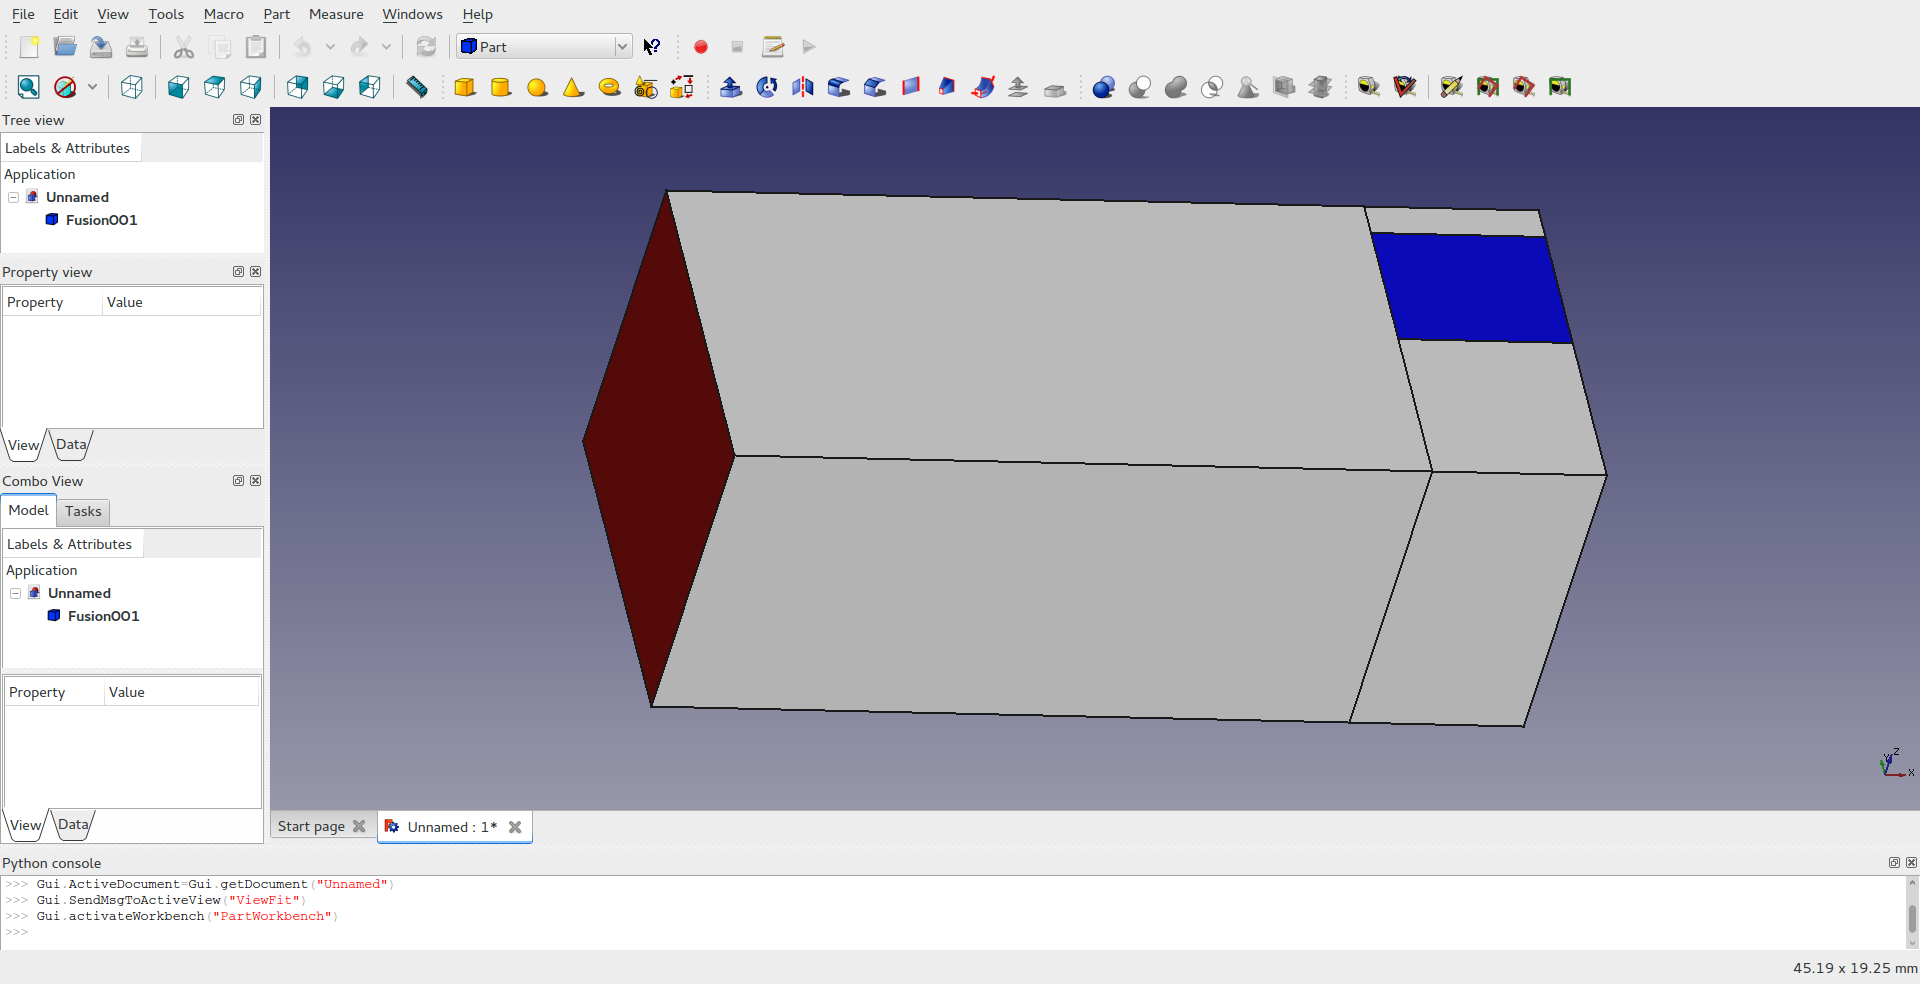
\includegraphics[width=.3\textwidth]{Pictures/TopOp/CantileverFCAD3.png}
%\caption{Color faces in FreeCAD}
%\label{fig: FreeCADColoring}
%\end{figure}
%\end{overlayarea}
%\end{minipage}
%\begin{minipage}{0.3\textwidth}
%\begin{overlayarea}{\textwidth}{.9\textheight}
%\begin{figure}[htp]
%	\centering
%	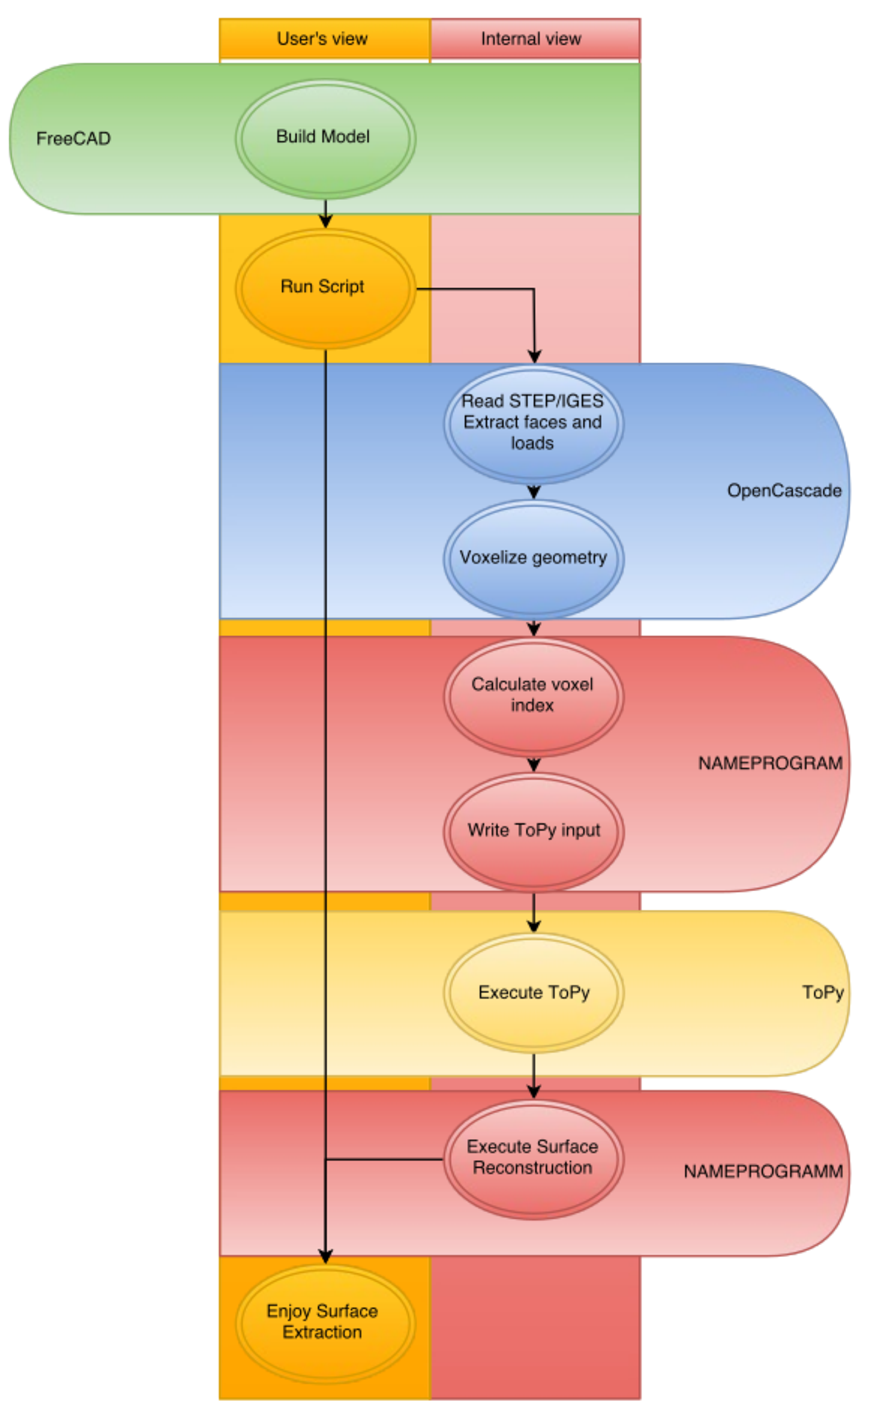
\includegraphics[scale=.25]{Pictures/TopOp/FlowChart/FlowDiagram2.pdf}
%\end{figure}
%\end{overlayarea}
%\end{minipage}
%\end{frame}

\begin{frame}
\begin{overlayarea}{\textwidth}{.9\textheight}
%\visible<1>{
\begin{tikzpicture}[spy using outlines={rectangle,lens={scale=2}, height=2cm,width=6cm, connect spies}]
\node[inner sep=0pt] (userView) at (0,0)
    {
\includegraphics[scale=0.23]{Pictures/TopOp/FlowChart/UserView.png}};
\node[inner sep=0pt, right of=userView] (internalView)
    {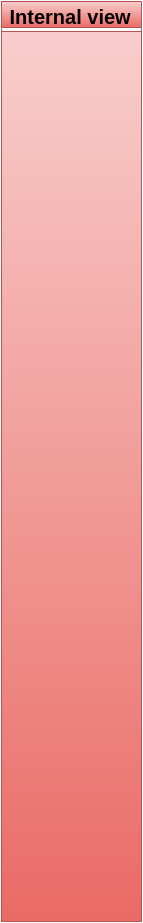
\includegraphics[scale=0.23]{Pictures/TopOp/FlowChart/InternalView.png}};
\visible<2->{
\node[inner sep=0pt] (FreeCAD) at (-0.15,3)
    {
\includegraphics[scale=0.23]{Pictures/TopOp/FlowChart/ModelFreeCAD.png}};
}
\visible<3>{
\spy [blue,visible on=<3>] on ([xshift=-0.2cm]FreeCAD)
             in node [left] at (9.2,2.6);

\node[draw,text width=7.1cm] at (5.7,-0.6) {
	%\footnotesize{
	\begin{itemize}
	\item Model geometry in your favorite CAD tool % (FreeCAD, OpenSCAD)
	\item Colour faces for boundary conditions% are applied
	\begin{itemize}
	%\footnotesize{
		\item[\textcolor{red}{Red}] Fixture
		\item[\textcolor{green}{Green}] Active
		\item[\textcolor{red}{R}\textcolor{green}{G}\textcolor{blue}{B}] RGB value in $[0 \leq \text{\textcolor{red}{R}} < 255,0 \leq \text{\textcolor{green}{G}} < 255,0 \leq \text{\textcolor{blue}{B}} < 255]$ for load vector
	%	}
	\end{itemize}
	\item Save model as \texttt{STEP with Colours} and \texttt{IGES with Colours}
	\end{itemize}
	%}
	};

}
\visible<4>{
\spy [blue,visible on=<4>] on ([xshift=-0.2cm]FreeCAD)
             in node [left] at (9.2,2.6);
%\draw[<->,thick] (userView.south east) -- (internalView.north west)
%    node[midway,fill=white] {whut};
%\end{tikzpicture}

\node[draw,text width=7.1cm] at (5.7,-1.2) {
\begin{figure}[htp]
\centering
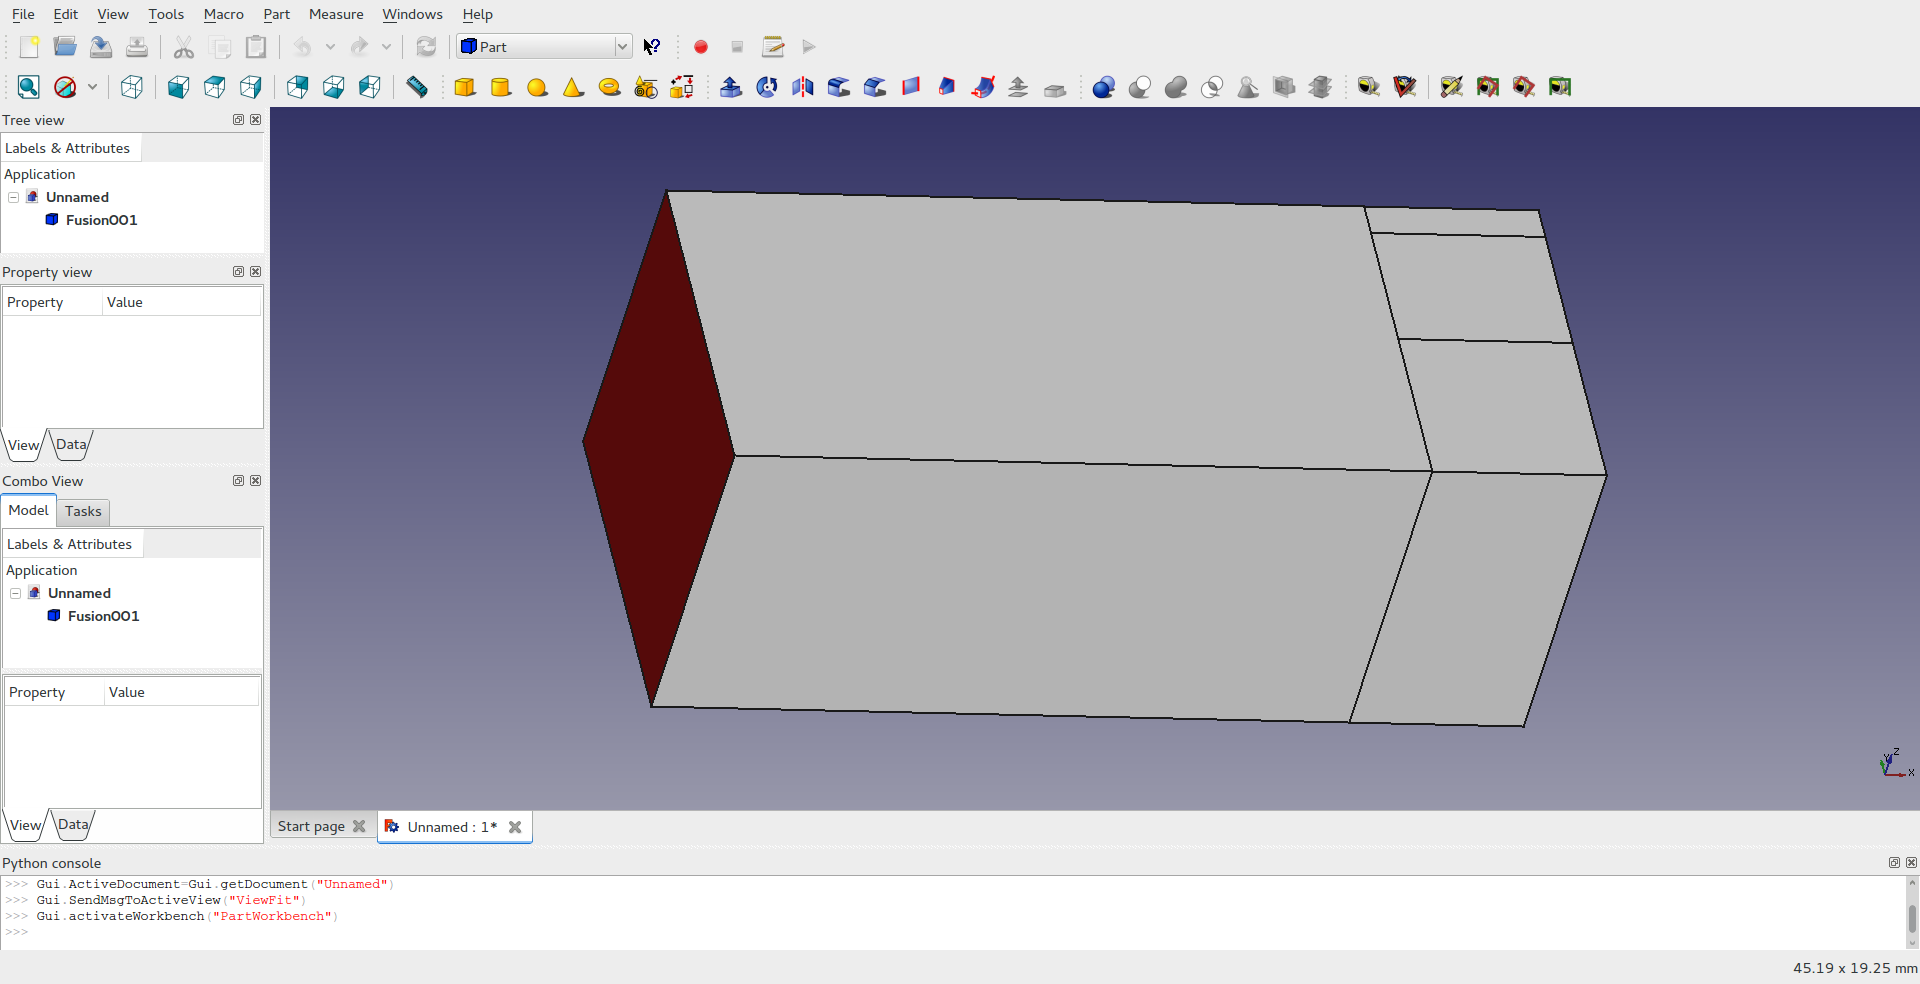
\includegraphics[width=.45\textwidth]{Pictures/TopOp/CantileverFCAD1.png}\hfill
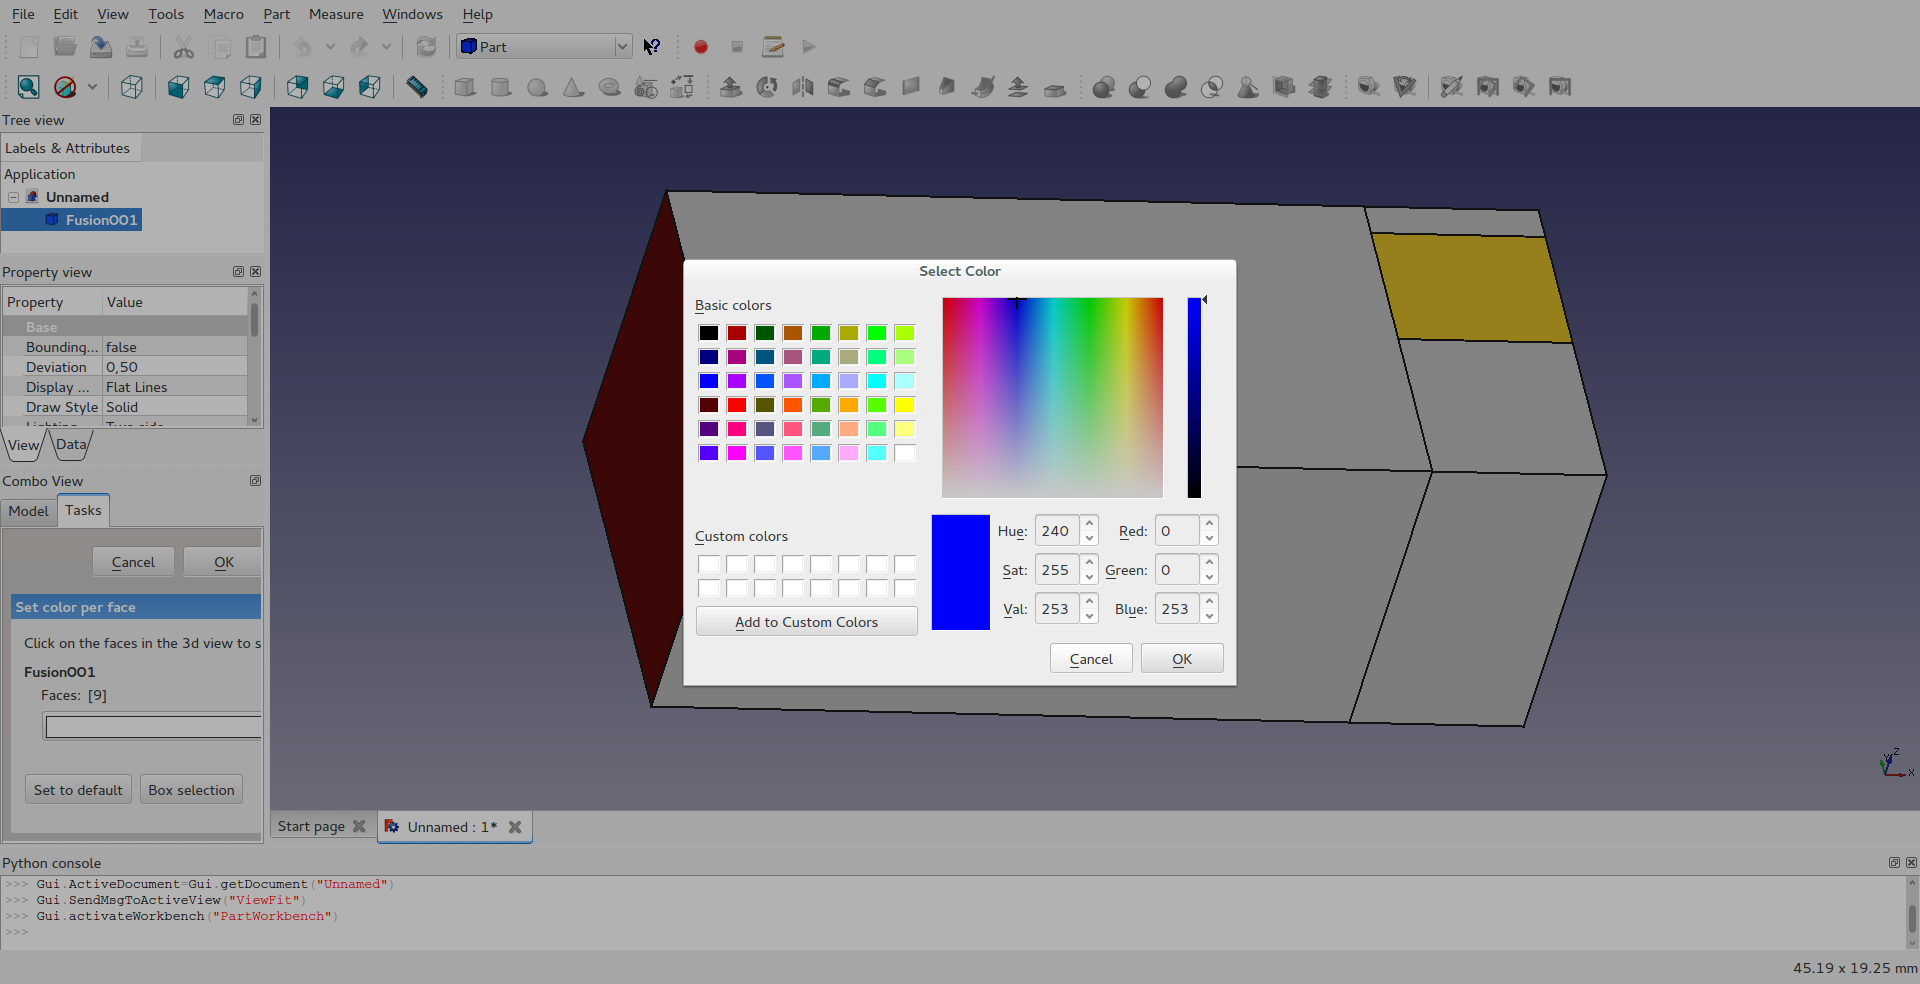
\includegraphics[width=.45\textwidth]{Pictures/TopOp/CantileverFCAD2.png}\\
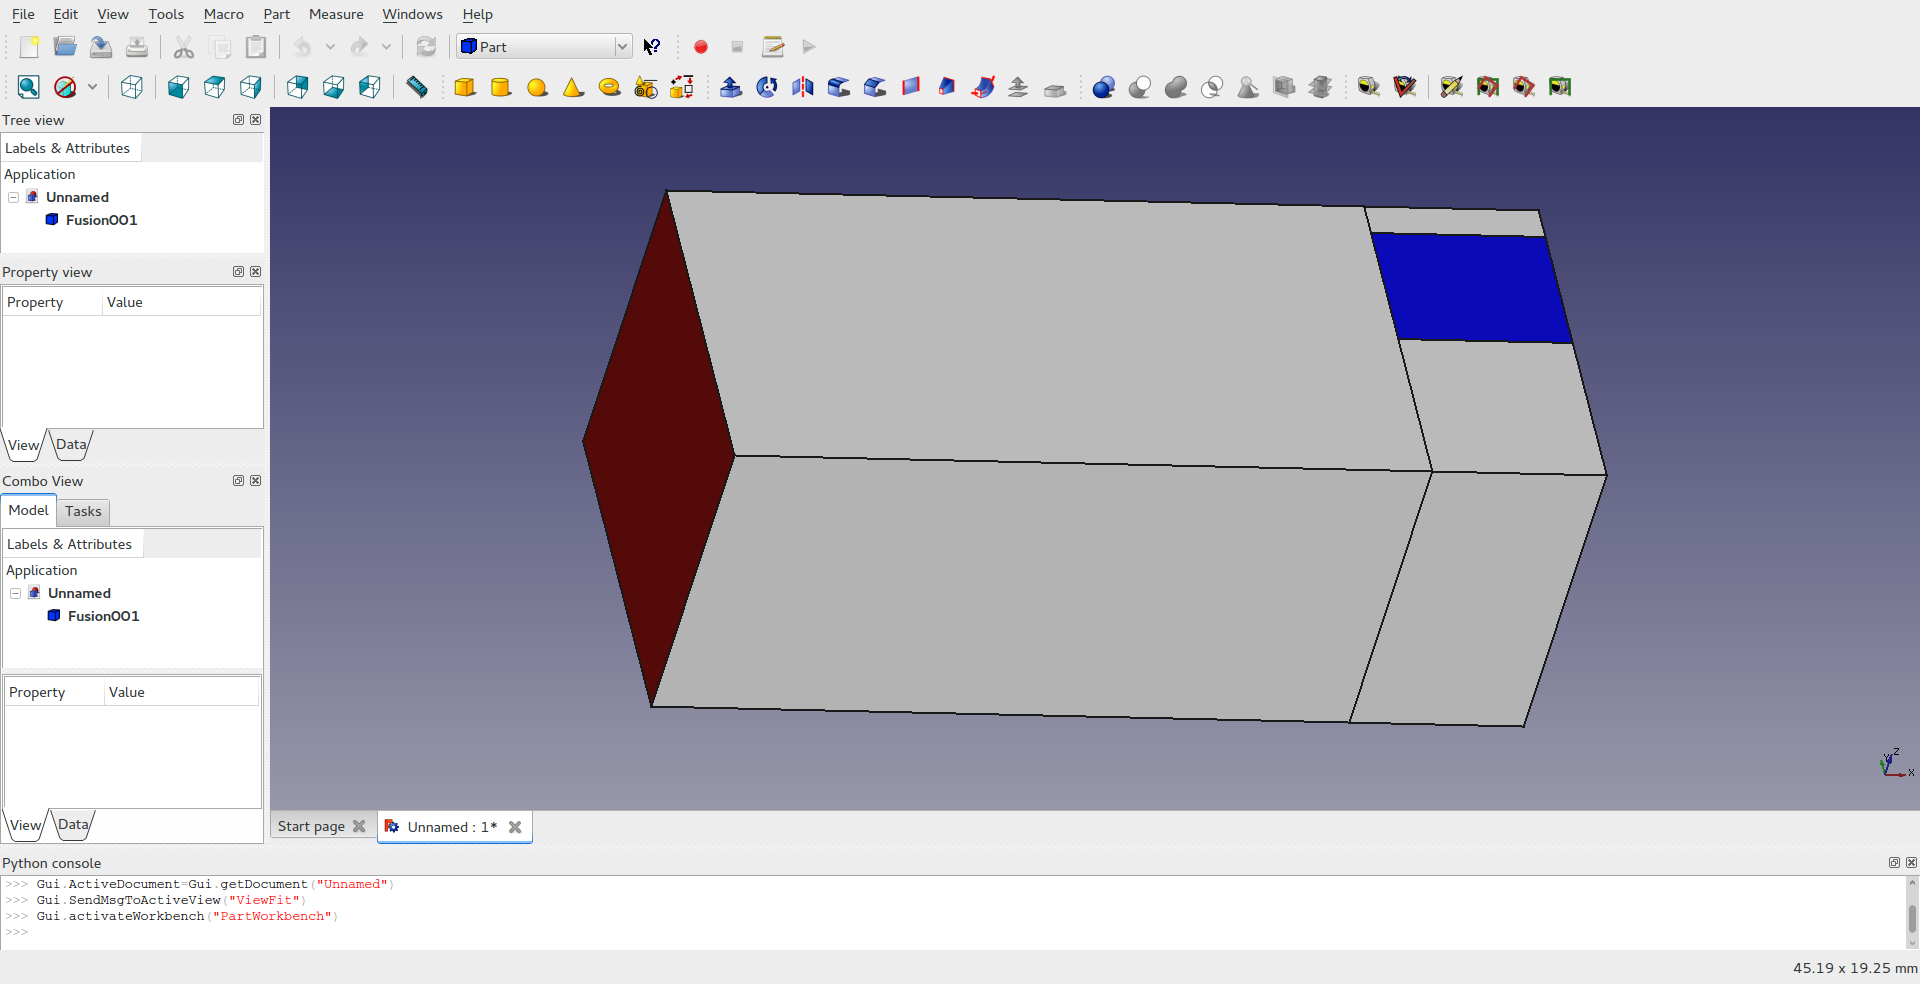
\includegraphics[width=.45\textwidth]{Pictures/TopOp/CantileverFCAD3.png}
\caption{Color faces in FreeCAD}
\end{figure}
	};

}
\visible<5->{
\node[inner sep=0pt] (RunScript) at (-0.15,2.3)
    {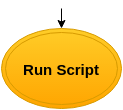
\includegraphics[scale=0.23]{Pictures/TopOp/FlowChart/RunScript.png}};
}
\visible<6>{
\spy [blue,visible on=<6>] on ([yshift=-0.2cm]RunScript)
             in node [left] at (9.2,2.6);
\node[draw,text width=7.1cm] at (5.7,-0.6) {
	$\rightarrow$ Run \\ \texttt{CADTopOpt filedir filename force{\_}scaling refinement}
	};
}
%\visible<7->{
%\node[inner sep=0pt] (EnjoySurface) at (-0.15,-0.9)
%    {
\includegraphics[scale=0.23]{Pictures/TopOp/FlowChart/EnjoySurfaceUser.png}};
%}
%\visible<8>{
%\spy [blue,visible on=<8>] on ([yshift=-2.5cm]EnjoySurface)
%             in node [left] at (8.5,3);
%\node[draw,text width=7.1cm] at (5.7,-0.6) {
%			\begin{figure}[htp]
%			\centering
%			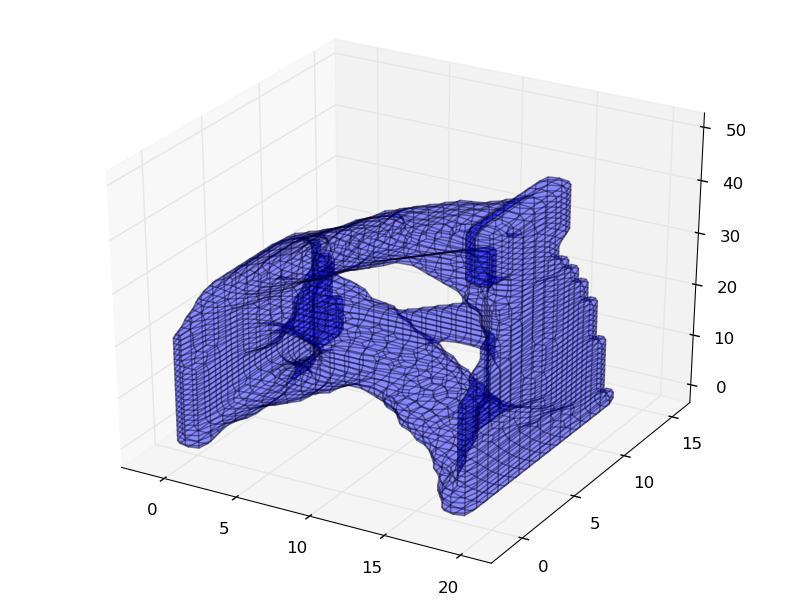
\includegraphics[scale=0.15]{Pictures/TopOp/SurfaceExtraction1.png}
%			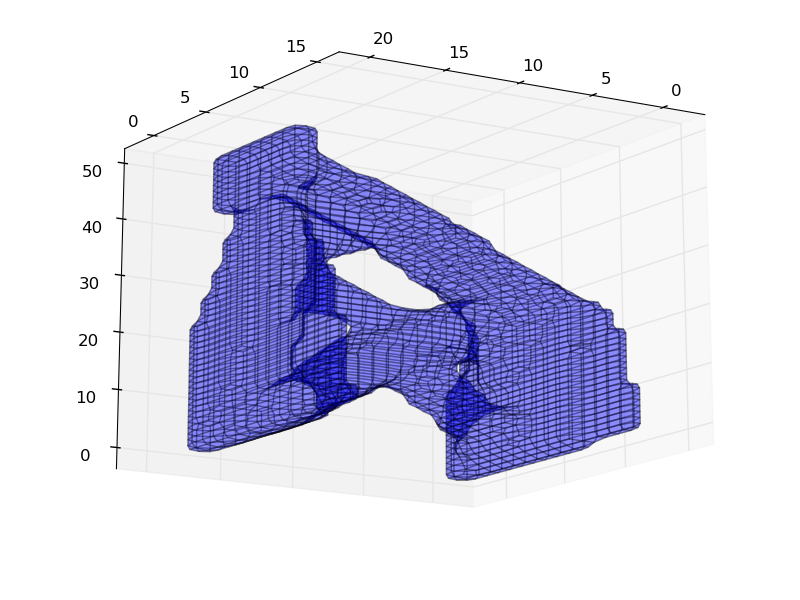
\includegraphics[scale=0.15]{Pictures/TopOp/SurfaceExtraction3.png}
%			\caption{Surface extraction for Cantilever}
%			\end{figure}
%	};
%}
\end{tikzpicture}
\end{overlayarea}
\end{frame}

\begin{frame}
\begin{overlayarea}{\textwidth}{.9\textheight}
\begin{tikzpicture}[spy using outlines={rectangle,lens={scale=2}, height=2cm,width=6cm, connect spies}]
\node[inner sep=0pt] (userView) at (0,0)
    {
\includegraphics[scale=0.23]{Pictures/TopOp/FlowChart/UserView.png}};
\node[inner sep=0pt, right of=userView] (internalView)
    {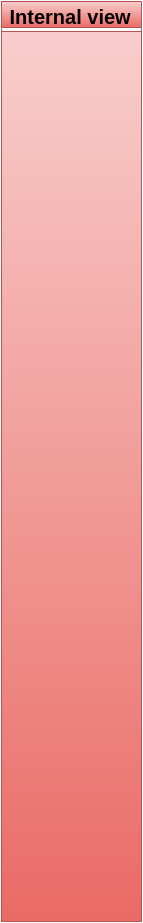
\includegraphics[scale=0.23]{Pictures/TopOp/FlowChart/InternalView.png}};
\node[inner sep=0pt] (FreeCAD) at (-0.15,3)
    {
\includegraphics[scale=0.23]{Pictures/TopOp/FlowChart/ModelFreeCAD.png}};
\node[inner sep=0pt] (RunScript) at (-0.15,2.3)
    {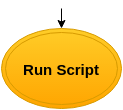
\includegraphics[scale=0.23]{Pictures/TopOp/FlowChart/RunScript.png}}; 
\visible<2->{
\node[inner sep=0pt] (OpenCascade) at (0.97,1.3)
    {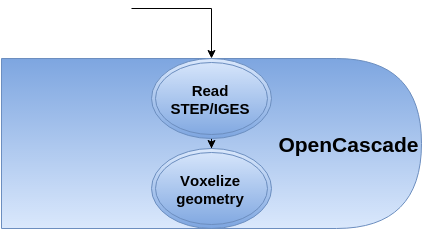
\includegraphics[scale=0.23]{Pictures/TopOp/FlowChart/OpenCascade.png}};
}
\visible<3>{
\spy [blue,visible on=<3>] on ([xshift=0.4cm,yshift=0.1cm]OpenCascade)
             in node [left] at (9.2,2.6);
\node[draw,text width=6.1cm] at (6.3,-0.6) {
	%\footnotesize{
	\begin{itemize}
		\item[] Read STEP and IGES file, extract colours and faces
		\begin{itemize}
			\item STEP holds the colours
			\item IGES holds the structure
		\end{itemize}
	\end{itemize}
	%}
};
}
\visible<4>{
\spy [blue,visible on=<4>] on ([xshift=0.4cm,yshift=-0.6cm]OpenCascade)
             in node [left] at (9.2,2.6);
\node[draw,text width=6.1cm] at (6.3,-1.2) {
	%\footnotesize{
	\begin{itemize}
		\item[] Voxelize faces using OpenCascade
	\end{itemize}
	
			\begin{figure}[htp]
				\centering
				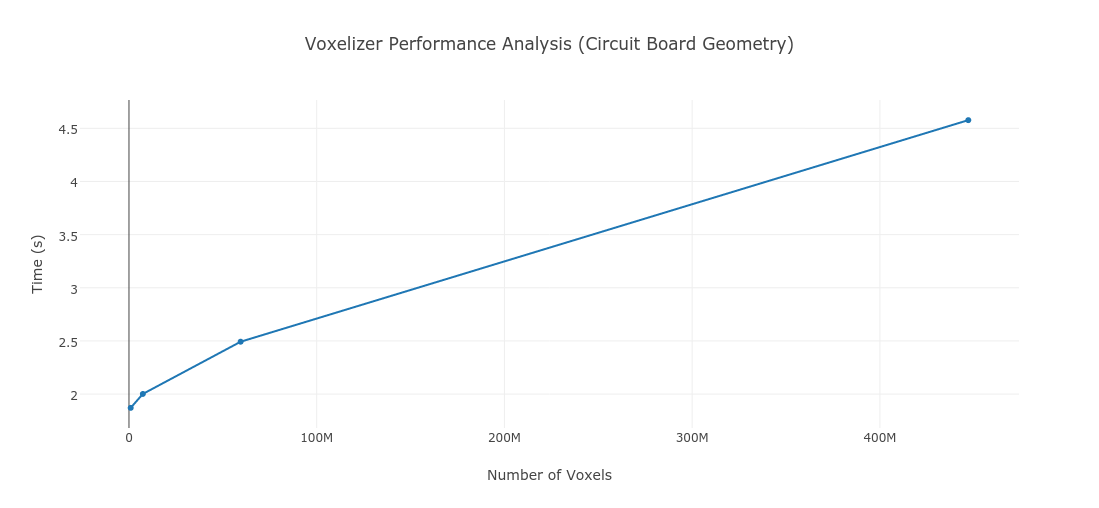
\includegraphics[scale=0.14]{Pictures/TopOp/VoxelizerScalingPlot.png}
				\caption{Scaling of voxelizer}
			\end{figure}
	%}
};
}
\visible<5->{
\node[inner sep=0pt] (Script1) at (0.97,-0.34)
    {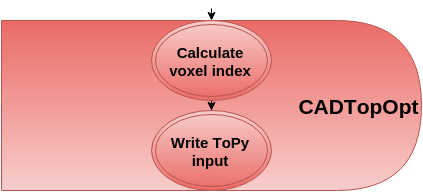
\includegraphics[scale=0.23]{Pictures/TopOp/FlowChart/Script1.png}};
}
\visible<6>{
\spy [blue,visible on=<6>] on ([xshift=0.4cm,yshift=0.3cm]Script1)
             in node [left] at (9.2,2.6);
\node[draw,text width=6.1cm] at (6.3,-1.2) {
	%\footnotesize{
		\begin{itemize}
			\item[] Different indexing for elements and nodes in ToPy
		\end{itemize}
	
			\begin{figure}[htp]
				\centering
				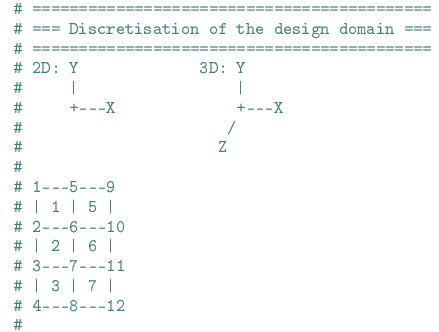
\includegraphics[scale=0.26]{Pictures/TopOp/ToPyIndexing.png}
				\caption{Indexing in ToPy [1]}
			\end{figure}
	%}
};
}
\visible<7>{
\spy [blue,visible on=<7>] on ([xshift=0.4cm,yshift=-0.4cm]Script1)
             in node [left] at (9.2,2.6);
\node[draw,text width=6.1cm] at (6.3,-1.2) {
	%\footnotesize{
		\begin{itemize}
			\item[] Each voxel index is specifically written
		\end{itemize}
		
			\begin{figure}[htp]
				\centering
				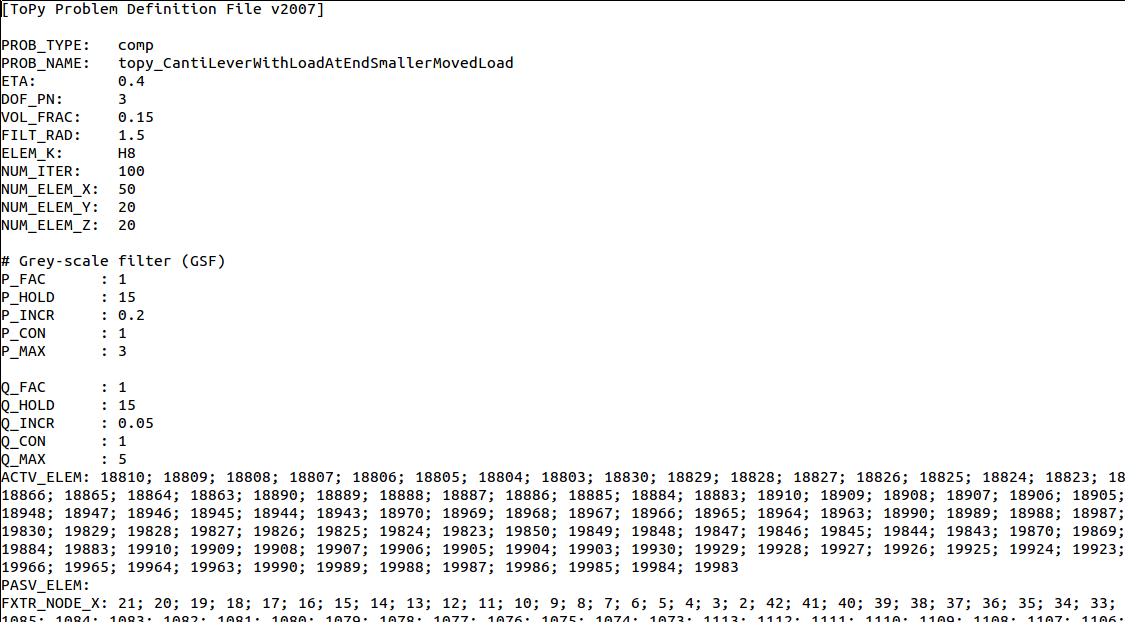
\includegraphics[scale=0.17]{Pictures/TopOp/ToPyInput.png}
				\caption{Script for ToPy}
			\end{figure}
	%}
};
}
\visible<8->{
\node[inner sep=0pt] (Topy) at (0.97,-1.591)
    {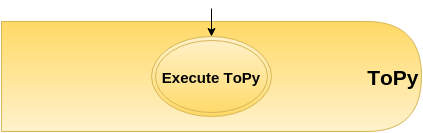
\includegraphics[scale=0.23]{Pictures/TopOp/FlowChart/TopyBold.png}};
}
\visible<9>{
\spy [blue,visible on=<9>] on ([xshift=0.4cm,yshift=-0.1cm]Topy)
             in node [left] at (9.2,2.6);
\node[draw,text width=6.1cm] at (6.3,-1.1) {
	%\footnotesize{
		\begin{itemize}
		\item[] Execute ToPy on the input file
		\end{itemize}	
			\begin{figure}[htp]
				\centering
				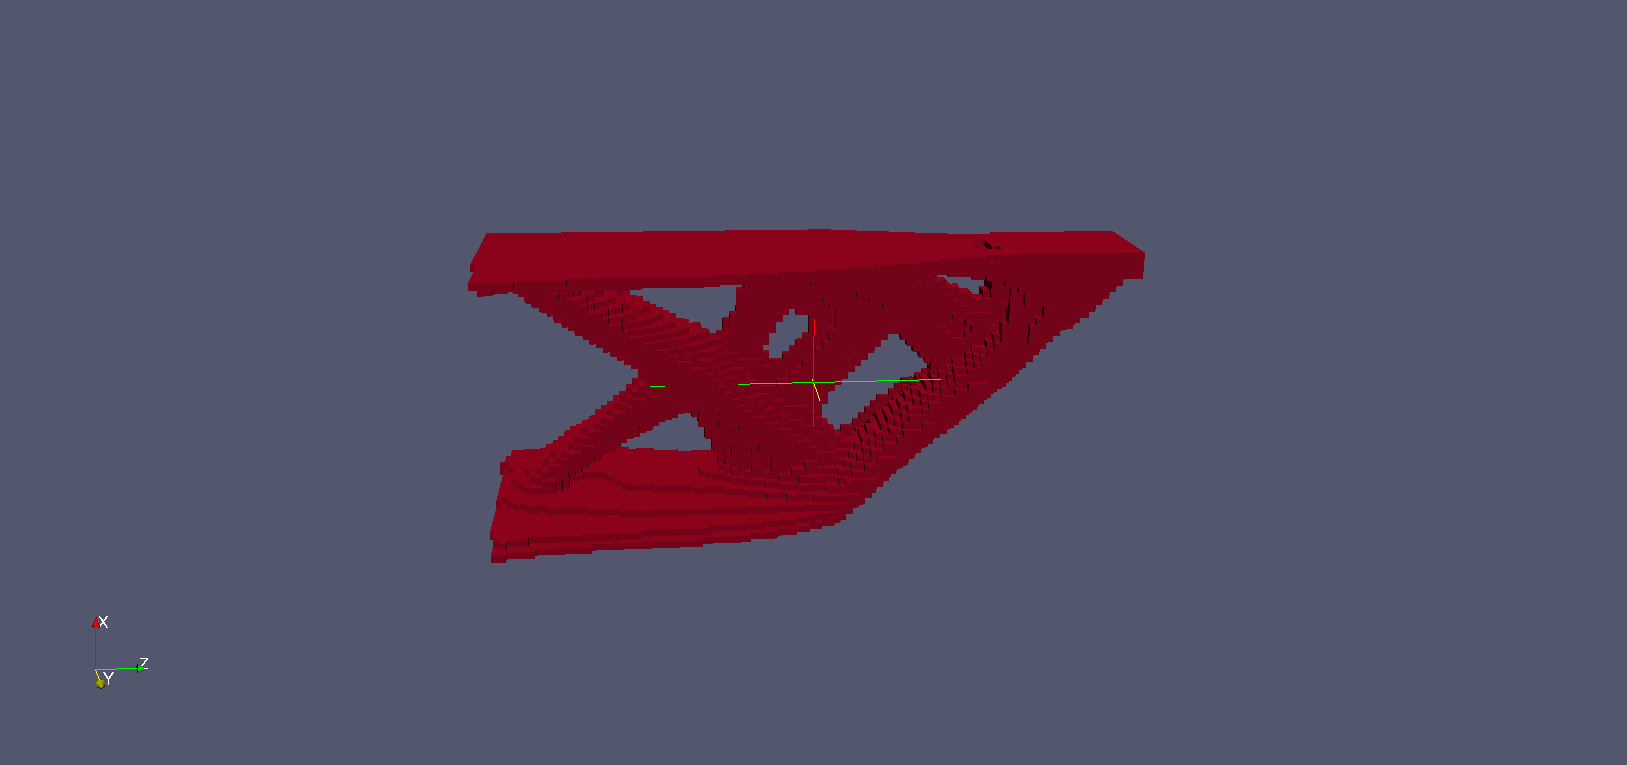
\includegraphics[scale=0.1]{Pictures/TopOp/CantileverToPy.png}
				\caption{ToPy Output}
			\end{figure}
	%}
};
}
\visible<10->{
\node[inner sep=0pt] (Script2) at (0.97,-2.507)
    {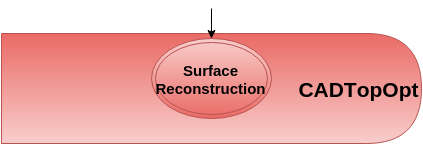
\includegraphics[scale=0.23]{Pictures/TopOp/FlowChart/Script2.png}};
}
\visible<11>{
\spy [blue,visible on=<11>] on ([xshift=0.4cm,yshift=-0.1cm]Script2)
             in node [left] at (9.2,2.6);
\node[draw,text width=6.1cm] at (6.3,-1.1) {
	%\footnotesize{
		\begin{itemize}
		\item[] Run dual contouring algorithm
		\end{itemize}	
			\begin{figure}[htp]
			\centering
			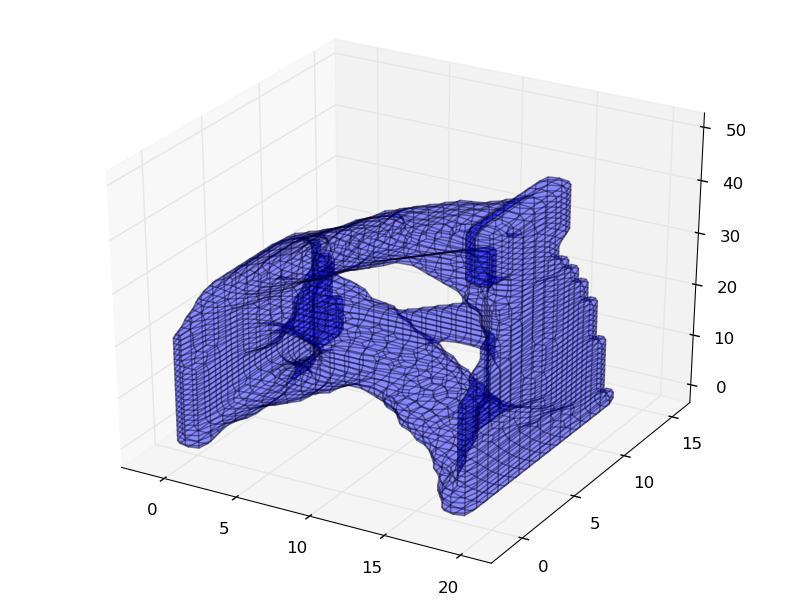
\includegraphics[scale=0.13]{Pictures/TopOp/SurfaceExtraction1.png}
			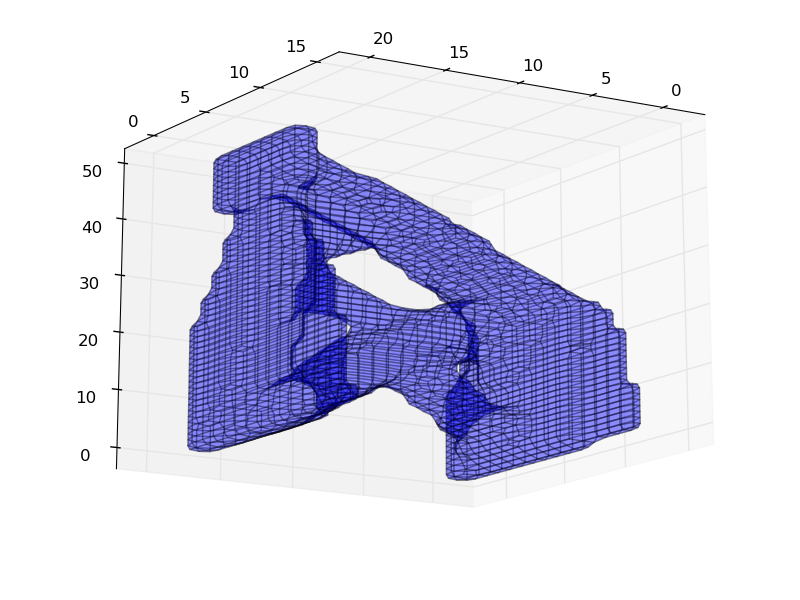
\includegraphics[scale=0.13]{Pictures/TopOp/SurfaceExtraction3.png}
			\caption{Surface extraction for Cantilever}
			\end{figure}
	%}
};
}
\visible<12->{
\node[inner sep=0pt] (EnjoySurfaceInternal) at (-0.038,-3.09)
    {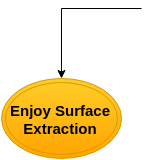
\includegraphics[scale=0.23]{Pictures/TopOp/FlowChart/EnjoySurfaceInternal.png}};
}
\visible<13>{
\node[draw,text width=4.5cm] at (5.8,1.1) {
	%\footnotesize{
		But what does the user see?
	%}
};
}
%\node[inner sep=0pt] (EnjoySurface) at (-0.15,-0.9)
%    {
\includegraphics[scale=0.23]{Pictures/TopOp/FlowChart/EnjoySurfaceUser.png}};
\end{tikzpicture}
\end{overlayarea}
\end{frame}

\subsection{User view}
\begin{frame}
\begin{overlayarea}{\textwidth}{.9\textheight}
\begin{tikzpicture}[spy using outlines={rectangle,lens={scale=2}, height=2cm,width=6cm, connect spies}]
\node[inner sep=0pt] (userView) at (0,0)
    {
\includegraphics[scale=0.23]{Pictures/TopOp/FlowChart/UserView.png}};
\node[inner sep=0pt, right of=userView] (internalView)
    {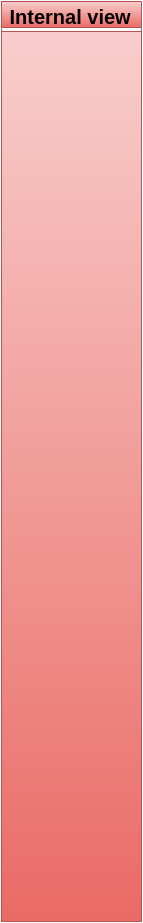
\includegraphics[scale=0.23]{Pictures/TopOp/FlowChart/InternalView.png}};
\node[inner sep=0pt] (FreeCAD) at (-0.15,3)
    {
\includegraphics[scale=0.23]{Pictures/TopOp/FlowChart/ModelFreeCAD.png}};    
\node[inner sep=0pt] (RunScript) at (-0.15,2.3)
    {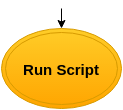
\includegraphics[scale=0.23]{Pictures/TopOp/FlowChart/RunScript.png}}; 
\node[inner sep=0pt] (EnjoySurface) at (-0.15,-0.9)
    {
\includegraphics[scale=0.23]{Pictures/TopOp/FlowChart/EnjoySurfaceUser.png}};
\node[draw,text width=4.5cm] at (5.8,1.1) {
	%\footnotesize{
		But what does the user see?
	%}
};
\end{tikzpicture}
\end{overlayarea}
\end{frame}

%\subsection{The internal view2}
%\begin{frame}{The internal view DRAFT}
%\begin{minipage}{0.65\textwidth}
%\begin{overlayarea}{\textwidth}{.9\textheight}
%\begin{itemize}
%	\item The pipeline:
%	\begin{enumerate}
%		\only<1> {
%		\item Read STEP and IGES file, extract colours and faces
%		\item Voxelize faces using OpenCascade
%		\item Calculate index for each voxel for ToPy
%		\item Write ToPy input file
%		\item Execute ToPy on the input file
%		\item Execute Surface Reconstruction on ToPy vtk output
%		}		
%		\only<2> {
%		\item Read STEP and IGES file, extract colours and faces
%		\begin{itemize}
%			\item STEP file holding the colours
%			\item IGES holding the structure
%		\end{itemize}
%		}
%		\only<3> {
%		\item Read STEP and IGES file, extract colours and faces
%		\item Voxelize faces using OpenCascade
%		\begin{itemize}
%			\item Included open cascade voxelizer
%			\begin{figure}[htp]
%				\centering
%				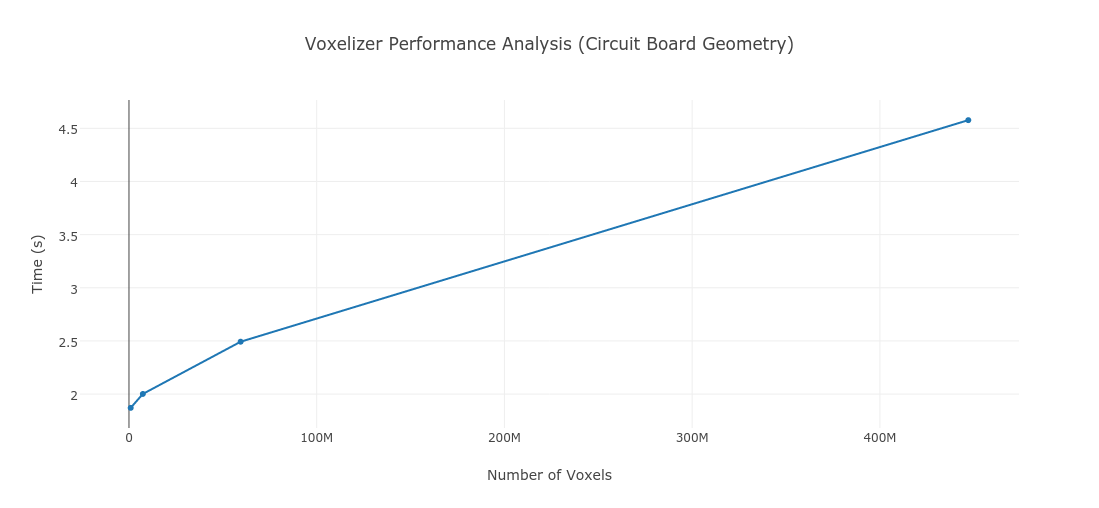
\includegraphics[width=.4\textwidth]{Pictures/TopOp/VoxelizerScalingPlot.png}
%				\caption{Scaling of voxelizer}
%				\label{fig: VoxelScaler}
%			\end{figure}
%		\end{itemize}
%		}
%		\only<4> {
%		\item Read STEP and IGES file, extract colours and faces
%		\item Voxelize faces using OpenCascade
%		\item Calculate index for each voxel for ToPy
%		\begin{itemize}
%			\item Different indexing for elements and nodes in ToPy
%			\begin{figure}[htp]
%				\centering
%				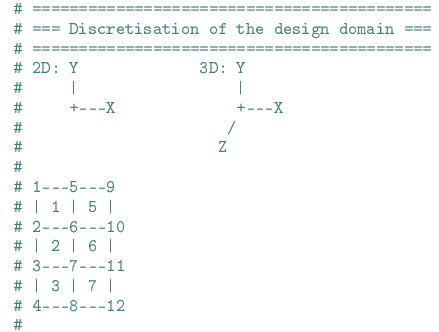
\includegraphics[width=.4\textwidth]{Pictures/TopOp/ToPyIndexing.png}
%				\caption{Indexing in ToPy}
%				\label{fig: TopyIndex}
%			\end{figure}
%		\end{itemize}
%		}
%		\only<5> {
%		\item Read STEP and IGES file, extract colours and faces
%		\item Voxelize faces using OpenCascade
%		\item Calculate index for each voxel for ToPy
%		\item Write ToPy input file
%		\begin{itemize}
%			\item Each voxel index is specifically written
%			\begin{figure}[htp]
%				\centering
%				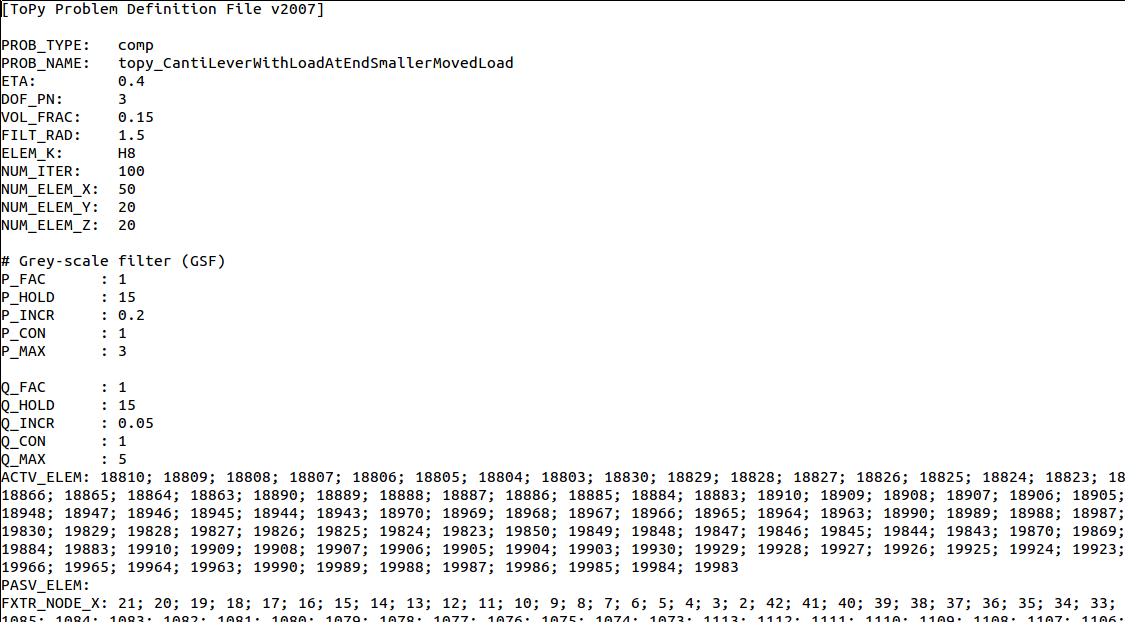
\includegraphics[width=.4\textwidth]{Pictures/TopOp/ToPyInput.png}
%				\caption{Script for ToPy}
%				\label{fig: TopyScript}
%			\end{figure}
%		\end{itemize}
%		}
%		\only<6> {
%		\item Read STEP and IGES file, extract colours and faces
%		\item Voxelize faces using OpenCascade
%		\item Calculate index for each voxel for ToPy
%		\item Write ToPy input file
%		\item Execute ToPy on the input file
%		\begin{itemize}
%			\item Topy runs....
%			\begin{figure}[htp]
%				\centering
%				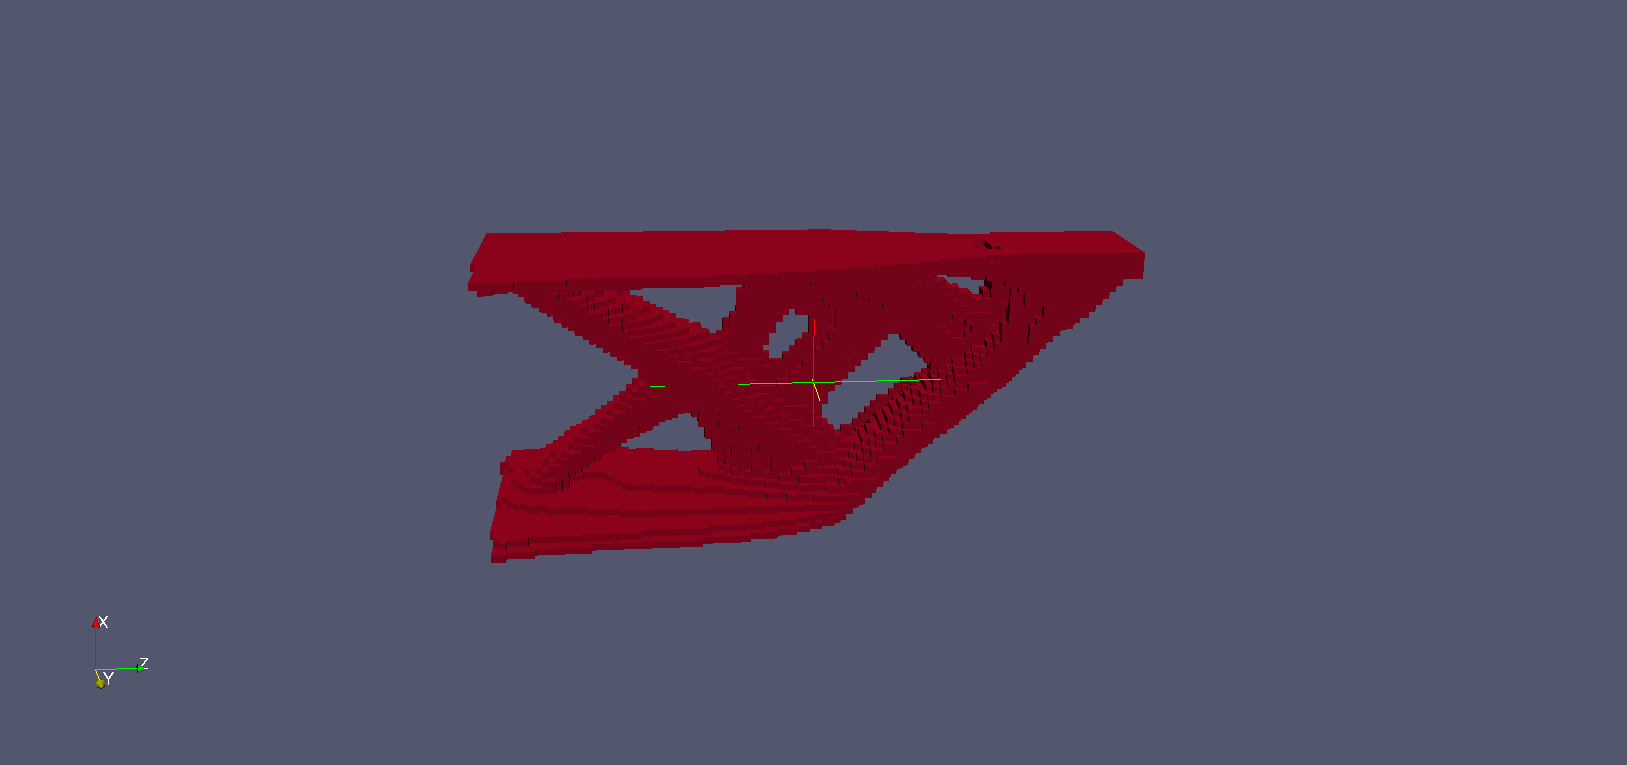
\includegraphics[width=.4\textwidth]{Pictures/TopOp/CantileverToPy.png}
%				\caption{ToPy Output}
%				\label{fig: topyoutput}
%			\end{figure}
%		\end{itemize}				
%		}
%		\only<7> {
%		\item Read STEP and IGES file, extract colours and faces
%		\item Voxelize faces using OpenCascade
%		\item Calculate index for each voxel for ToPy
%		\item Write ToPy input file
%		\item Execute ToPy on the input file
%		\item Execute Surface Reconstruction on ToPy vtk output
%		\begin{itemize}
%			\item Running dual contouring algorithm
%			\begin{figure}[htp]
%			\centering
%			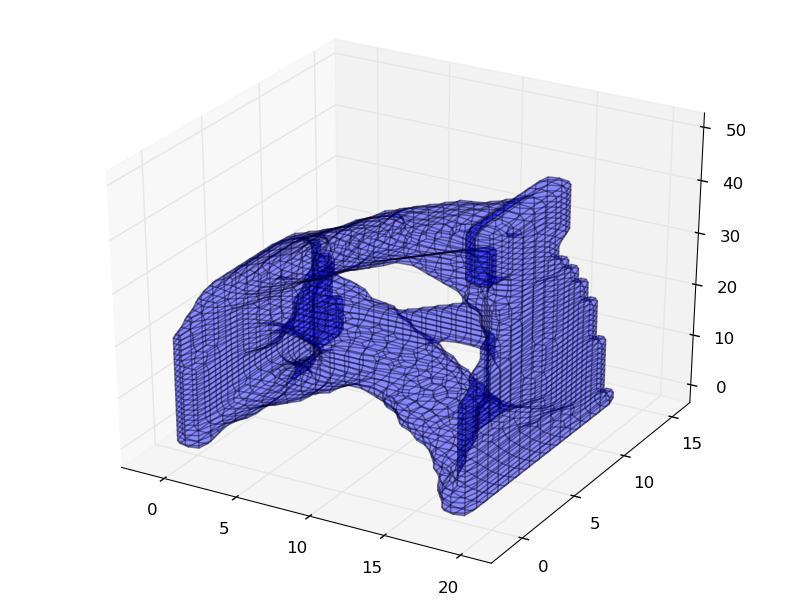
\includegraphics[scale=0.15]{Pictures/TopOp/SurfaceExtraction1.png}
%			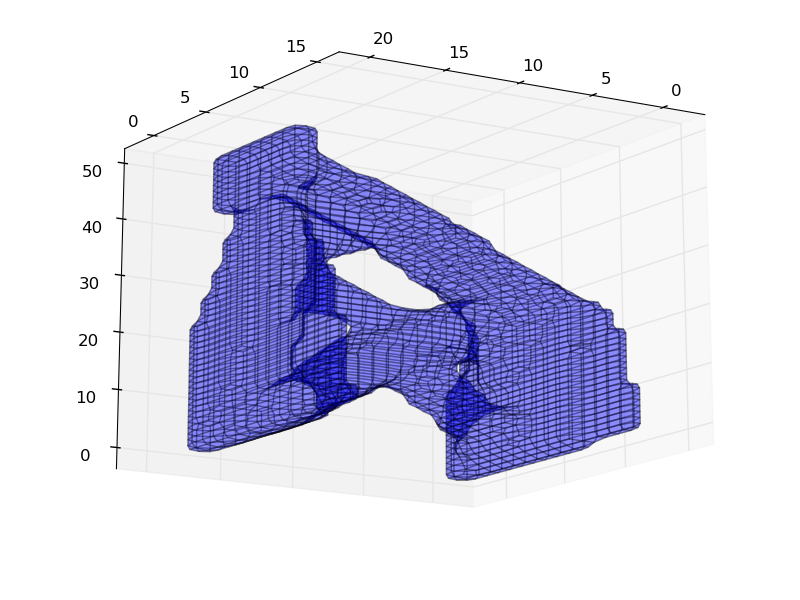
\includegraphics[scale=0.15]{Pictures/TopOp/SurfaceExtraction3.png}
%			\caption{Surface extraction for Cantilever}
%			\label{fig: SurfaceExtraction}
%			\end{figure}
%		\end{itemize}				
%		}
%	\end{enumerate}
%\end{itemize}
%\end{overlayarea}
%\end{minipage}
%\begin{minipage}{0.3\textwidth}
%\begin{overlayarea}{\textwidth}{.9\textheight}
%\begin{figure}[htp]
%	\centering
%	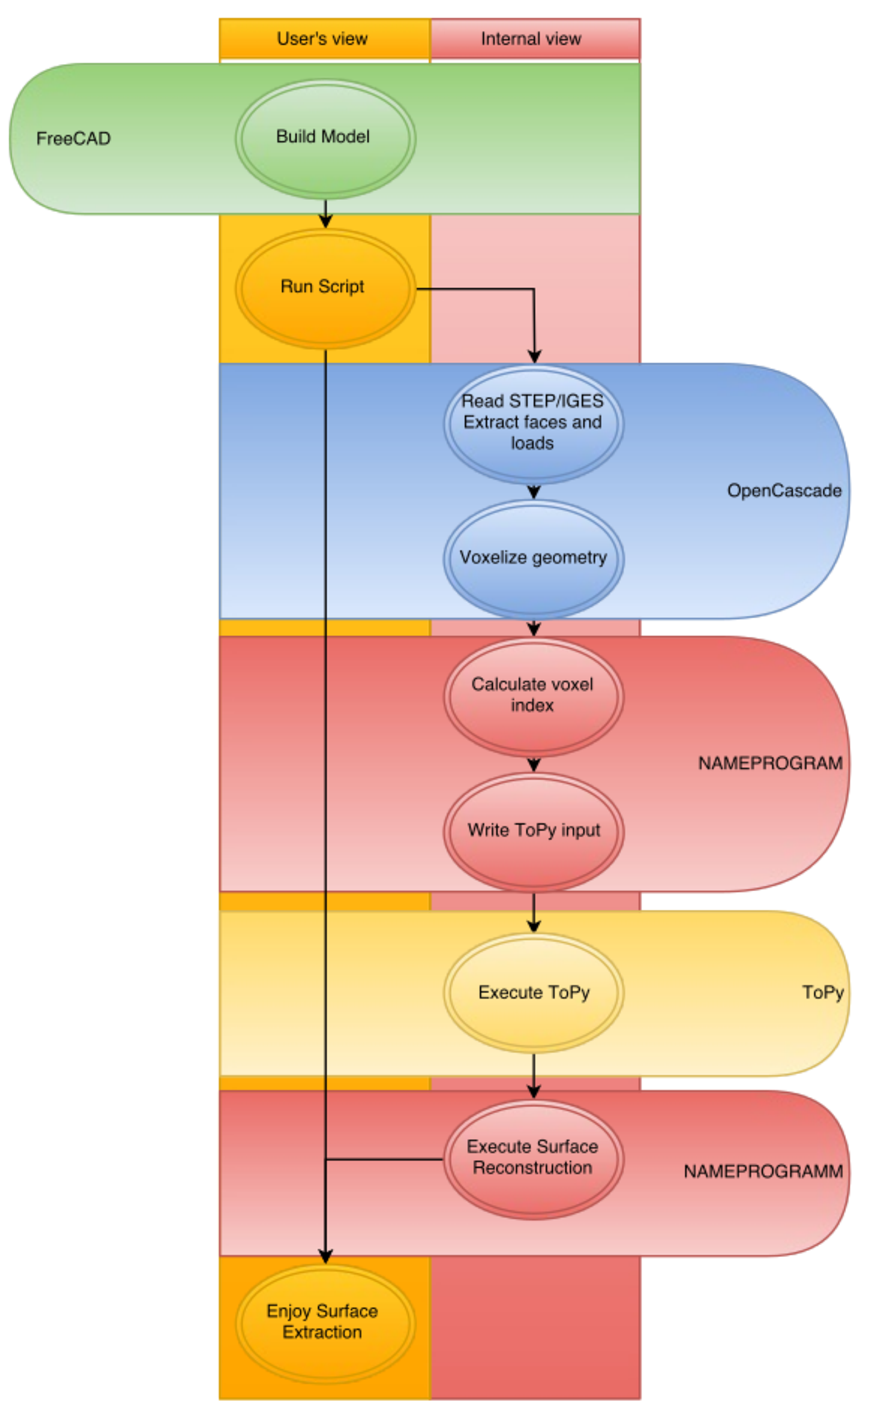
\includegraphics[scale=.25]{Pictures/TopOp/FlowChart/FlowDiagram2.pdf}
%\end{figure}
%\end{overlayarea}
%\end{minipage}
%\end{frame}